\chapter{Middle-level Intermediate Representation}
\label{chapter:mir-design}

This chapter describes SableWasm's middle-level intermediate representation
(MIR), which has a critical role in the entire compilation pipeline. The MIR
acts as a middle ground between the WebAssembly bytecode frontend and various
possible backends. Currently, SableWasm only implements one backend that
utilizes the LLVM compilation framework, but adding more backend support should
not require significant modification on the MIR. It also implements an
analysis and transformation framework where we perform several optimizations
over the MIR. We will first go over the overall design of the MIR, and
later move to the translation rules and analysis framework in the
chapter~\ref{chapter:mir-translation-optimization}. \\[12pt]


In the previous chapters, we covered the design of WebAssembly bytecode. A quick
reminder, WebAssembly is a stack-based intermediate representation (IR) where
all instructions operate over an implicitly declared operand stack. There are
several advantages of a stack-based IR. Perhaps the most important one is its
portability. A stack-based IR makes fewer assumptions on the machine than a
register-based one. One can even provide an implementation for a hypothetical
device with only one register. Another advantage is the code size. Experiments
show that, in general, a stack-based IR is smaller in size than its
corresponding registered version \cite{stack-and-register-vm}. When designing a
binary format that ships executables over the internet, the stack-based IR seems
to be a better choice for WebAssembly.

Nevertheless, there are no silver bullets: a stack-based IR design also has its
drawbacks. One of them is the difficulty faced when performing code analysis and
transformation over the module. As for each instruction, its operands implicitly
come from the stack; the value use-definition relationship between instructions
is not apparent to the analysis, and recovering such connection between
instructions from the IR is not a trivial task.

\begin{figure}
    \centering
    \lstinputlisting[
        language=SableWasmMIR,
        basicstyle=\linespread{0.8}\ttfamily,
        numbers=left
    ]{Code/4.MIR/fibonacci.mir}
    \caption{Fibonacci in translated SableWasm MIR}
    \label{fig:mir-fibonacci}
\end{figure}

On the other hand, we have the register-based intermediate representation,
commonly abstracted to assume an infinite number of registers and requiring a
register allocation algorithm to map them to actual, physical registers. For
each instruction in register-based IR, it has its operand encoded in the
instruction. Hence, the use-definition relationship will become explicit to the
analysis and transformation.

The main design goal for SableWasm MIR is to provide an analysis platform for
the entire compiler system. Thus, we implement our MIR as an infinite register
machine. We also take a traditional approach in various other aspects. For
example, instead of using the structured control flow similar to what
WebAssembly offers, we use \emph{control-flow graphs} (CFGs) to represent the
relationship between basic blocks. The SableWasm MIR is also in
\emph{single static assignment} (SSA) form \cite{ibm-ssa}, as covered in the
background chapter. The design for instruction and module-level entities in
SableWasm MIR is quite similar to what WebAssembly instruction offers. One can
view the SableWasm MIR as a mixture of the target LLVM intermediate
representation and the source WebAssembly bytecode. We also adopt several design
features from LLVM IR into MIR, such as automatically managed use-site lists,
which provide each AST node with an efficient way to access their use sites.
In SableWasm MIR, all elements are derived from the base class \texttt{ASTNode}
which implements these features that are helpful later in MIR analysis and
transformation.

Figure~\ref{fig:mir-fibonacci} shows a simple function that calculates Fibonacci
numbers with a recursive method in SableWasm MIR. With the help of the figure,
we will go through the detailed design of SableWasm later in the chapter. We
will first present the module-level entity and their initializer
expressions, such as functions, then move to the design of each instruction
defined in MIR.

\section{MIR Module Entities}
\label{section:mir-design-module-entities}

\begin{figure}
  \centering
  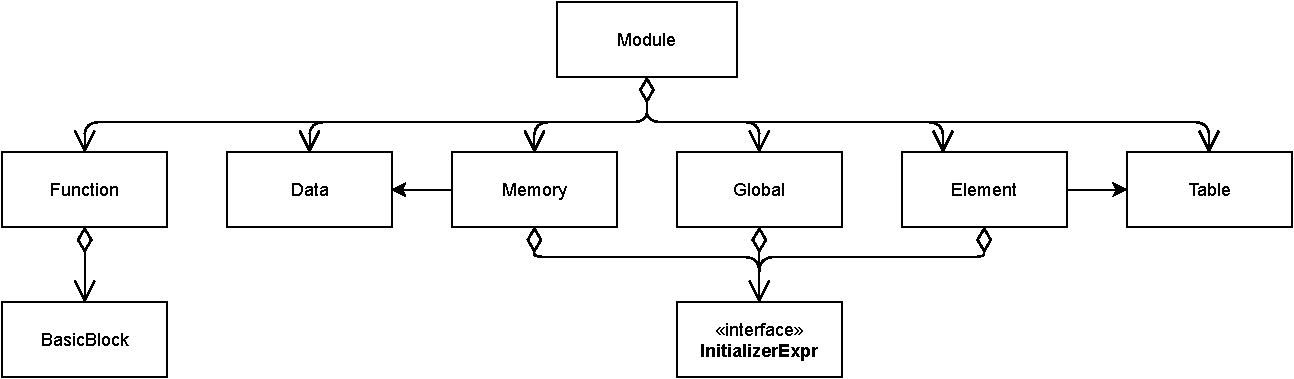
\includegraphics[width=\textwidth]{Images/4.MIR/module.pdf}
  \caption{SableWasm MIR Module-level entities}
  \label{fig:sablewasm-mir-module}
\end{figure}

SableWasm module-level entities are the top-level elements in a translation
module. They are direct implementations of the WebAssembly module entities
defined in the specification. Figure~\ref{fig:sablewasm-mir-module} presents a
general illustration of the SableWasm module-level entities. In this section,
we will cover the design of each entity and compare it with its WebAssembly
correspondent. All SableWasm module-level entities can optionally have import
and export annotates, except \texttt{data} and \texttt{element}. These
annotations correspond to the import and export entries defined in the
WebAssembly specification.

\paragraph{Function}
In figure~\ref{fig:mir-fibonacci}, we have a function definition at line 8. A
function declaration in SableWasm provides information about the type, local
variables, and name. A function definition should satisfy all the function
declaration requirements and, in addition, provide a function body using basic
blocks. The design of the function declaration and definition in SableWasm is
quite similar to that of WebAssembly. The only major difference is how to
represent the function body. We will come back to this in the later sections
within this chapter when we discuses the design of SableWasm MIR instructions.

\paragraph{Global}
SableWasm's global variable declaration and definition follow the design in
WebAssembly. In SableWasm, we relax several of the constraints defined in the
WebAssembly specification and its extensions. In the SIMD extension proposal,
the 128-bit vector type, \texttt{v128}, is only suitable within the function
body. There is no direct way to pass a vector value to the host environment, as
there is a lack of standard representation for 128-bit packed vectors in
JavaScript \footnote{This might subject to change in the future.}. In SableWasm,
we treat all primitive types uniformly. Thus, a global variable can contain an
integral value, a floating-point value, or even a packed SIMD vector. The type
for the SableWasm MIR global variable follows the specification in WebAssembly;
it consists of a value type and a constness modifier. In
figure~\ref{fig:mir-fibonacci}, we have a global variable definition at line 6,
which introduces a mutable 32-bit integral value. All global variable
definitions in SableWasm must provide a value initialization via an initializer
expression. In SableWasm MIR, all initialization expressions are constant
expressions, meaning that the host system can deduce the resulting values at the
module initialization phase. At runtime, the host system will first evaluate
these expressions and then initialize the global variables accordingly.
We will come back to the initialization expressions in detail later in this
chapter.

\paragraph{Memory and Data}
Memory and Data are implementations of the WebAssembly linear memory and its
initializer, respectively. One might think that there is no need to separate the
memory initializer from the memory entity definition, as in WebAssembly
specification, all data section entries must provide a valid linear memory
index. In the early version of SableWasm, we indeed adopt such implementation.
However, this approach might be subject to a significant change in an extension
that might soon merge to the WebAssembly specification. The WebAssembly bulk
memory operation extension proposal \footnote{WebAssembly bulk memory
  operations: \\\url{https://github.com/WebAssembly/bulk-memory-operations}}
introduces new instructions, such as \texttt{memory.fill} that directly refers
to a data section segment. Moreover, the proposal relaxes the constraints on the
linear memory index. Now the index can behave as a flag indicating whether the
data segment itself is active or not and no longer serves as a linear memory
index. Hence, to make our framework `futureproof', we separate linear memory
declarations from their initializers. Figure~\ref{fig:mir-fibonacci} presents a
linear memory definition at line 2. SableWasm memory entities also adopt
WebAssembly's linear memory type. The type consists of a pair of unsigned
integers, indicating the lower bound and upper bound of the memory size in
WebAssembly pages. The example above defines a memory with a minimal size of 2
pages, 128KiB, and exports it under the name `memory'. It, however, does not
provide any example for data initializers, although they are quite easy to
understand: a data initializer is essentially a binary chunk with an
initialization offset, and is semantically equivalent to a data section entry
in an ELF file.

\paragraph{Table and Element}
SableWasm's table and element entity implement the indirect table and its
initializer, namely element segment, accordingly. They follow the same principle
as the memory and data entity in the previous section. Currently, like a data
segment entry, WebAssembly's element section entry must refer to a valid
indirect table via an index. In the future, this may also subject to change. The
WebAssembly reference types extension proposal \footnote{WebAssembly reference
  types: \url{https://github.com/WebAssembly/reference-types}} introduces
instructions such as \texttt{table.fill} that are able to have direct access to
element segment initializers. \texttt{table.fill} instruction is similar to
\texttt{memory.fill} defined in the bulk memory operation extension. It will
copy a sequence of compile-time defined function pointers into an indirect table
at runtime. Thus, when we design our table entity, we also split the
declarations from their initializers. The type for table entity is the same as
the table type in WebAssembly. It consists of a pair of unsigned integers,
indicating the lower bound and upper bound for the number of function pointers
stored in the indirect table. In SableWasm MIR, we treat memory entities and
table entities as black boxes, and its concrete implementation is deferred to
the backend. In the example shown in figure~\ref{fig:mir-fibonacci}, the module
defines a table entity at line 4 that stores exactly one function pointer. Note
that the table entity does not require users to initialize the value for all
entries. The table entity default initializes all entries to null pointers.

In this section, we covered the design for module-level entities in SableWasm.
They are pretty similar to the those defined in the WebAssembly specification.
In the next section, we will move the design of SableWasm initialization
expressions.
\subsection{MIR Initializer Expressions}

\begin{figure}
  \centering
  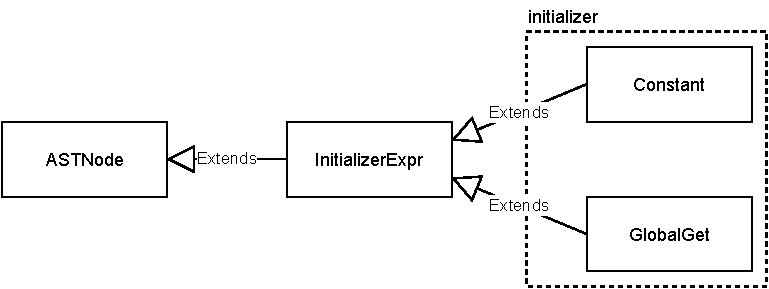
\includegraphics[width=0.85\textwidth]{Images/4.MIR/initalizer-expression.pdf}
  \caption{SableWasm MIR Initializer Expression}
  \label{fig:sablewasm-mir-initializer-expression}
\end{figure}

WebAssembly defines a particular form of expression for initialization, namely
constant expressions. They can appear in three locations in the current
specification. First, global variables declaration can contain constant
expression as their initialization values. Additionally, data section entries
and element section entries can have constant expressions as the offsets for
their initialization payload. In SableWasm MIR, we define initializer
expressions that act similar to what constant expressions do in WebAssembly.
Figure~\ref{fig:sablewasm-mir-initializer-expression} gives a general
illustration about SableWasm MIR initializer expressions. The initializer
expressions are quite simple. In the current WebAssembly and SableWasm, an
initializer expression can be either a constant value or refer to an imported
global via \texttt{GlobalGet} instruction. Hence, in principle, currently,
a SableWasm MIR initializer expression is essentially a single instruction. In
the future, one may generalize such constraints by allowing more complex
constructs in initializer expressions.

\paragraph{Constant}
The \texttt{Constant} instruction represents a single constant value for the
initializer expression. In WebAssembly, a constant value can be one of the
following: a 32-bit or 64-bit integer, a floating-pointer number, or a 128-bit
SIMD vector \footnote{With WebAssembly SIMD128 extension}, and the specification
encodes the type within the instruction opcode. Hence, there are multiple
instructions in WebAssembly to introduce a constant. In SableWasm, we do not
encode the type into the opcode, and \texttt{Constant} instruction is the only
instruction that takes care of the task. In figure~\ref{fig:mir-fibonacci}, we
have a constant initializer at line 6 that initializes the value of the global
to a 32-bit integer with a value that equals 66560. When querying the type of a
\texttt{Constant} instruction, SableWasm will infer it according to its payload
constant.

\paragraph{GlobalGet}
The \texttt{GlobalGet} instruction is exactly same as the WebAssembly's
\texttt{global.get} in terms of execution semantics. The WebAssembly
specification allows any initializer expression to refer to an imported
\footnote{This might subject to change in the future version of WebAssembly}
global value. As these values are initialized before entering the module,
reading their value is always valid during module initialization. The example
in figure~\ref{fig:mir-fibonacci} does not provide an example of
\texttt{GlobalGet} as an initializer expression, as they are less frequently
used compared to constant initializer expression, especially for global values.
However, in some ABI implementations, data section entries and element section
entries require reading from global values serving as base pointers. SableWasm
also infer the type for \texttt{GlobalGet} initializer expression in a similar
fashion as \texttt{Constant}. In this case, the type of instruction is the same
as the referred global variable without the `constant' modifier.

In this section, we covered the design and implementation of initializer
expressions in SableWasm. They are pretty simple in the current design. We will
now move to the next part in the SableWasm design, the MIR instructions.
\section{MIR Instructions}

SableWasm MIR uses a control-flow-graph (CFG) based representation in
\emph{static single assignment} (SSA) form to represent code body in function
definitions. We have provided an introduction to CFG and SSA in the background
chapter. Here is a quick recap. CFG splits the control flow within the function
into basic blocks. A basic block represents the most extended instruction
sequence without control flow transfer, such as branching. Note that for
function calls, we take a similar approach to that of LLVM. We will come back
to this in detail later in this section. Additionally, SSA requires that all
values must have unique definition sites. Hence, in SSA form, the
use-definition chain is trivial to compute, while in a traditional CFG, one
would need to extract this from the graph with the help of a \emph{reaching
  definition} analysis. The SableWasm MIR instruction set is similar to
WebAssembly bytecode in terms of semantics for most of the instructions.
However, it operates over an infinite register machine instead of a
stack-based machine, and in some cases, semantics differ in order to keep the
size of the SableWasm instruction minimal. In this section, we will cover the
design and implementation of SableWasm MIR instructions. The following section
will cover the translation strategy between WebAssembly bytecode and the
SableWasm MIR and instruction reduction rules.
Figure~\ref{fig:sablewasm-mir-inst} provides a general illustration of the
design of the SableWasm MIR instruction set. The SableWasm MIR instruction set
can currently cover all the instructions defined in WebAssembly specification,
including several extensions such as multivalue and SIMD vector operations.

\begin{figure}
  \centering
  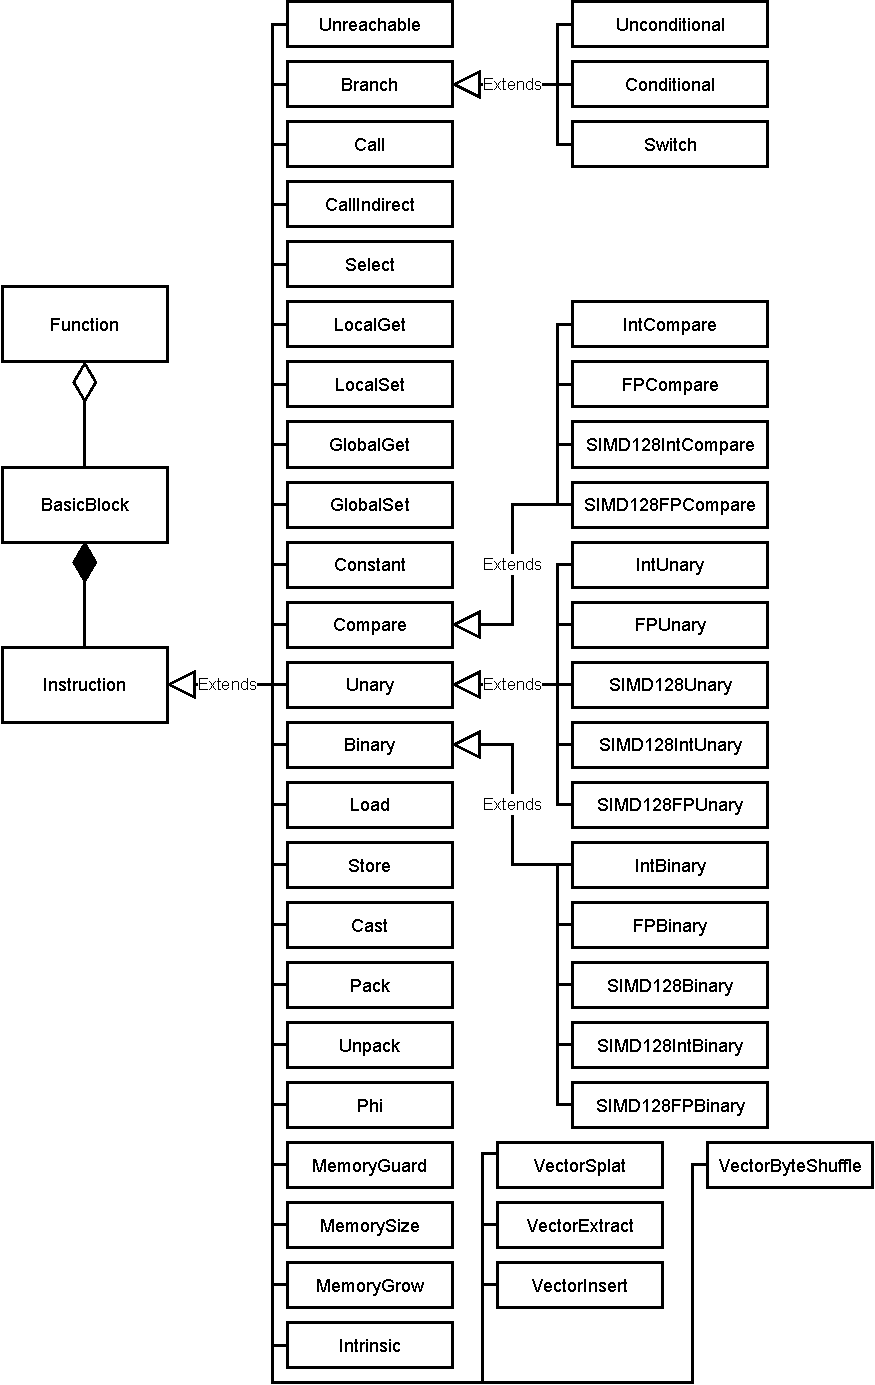
\includegraphics[width=0.8\textwidth]{Images/4.MIR/sablewasm-instruction.pdf}
  \caption{SableWasm MIR Instructions}
  \label{fig:sablewasm-mir-inst}
\end{figure}

\paragraph{Terminating instructions}
As discussed above, SableWasm splits the function control flow into basic
blocks containing the maximum number of consecutive instructions without
control flow transfer. In addition, SableWasm, similar to many other SSA form
instruction sets, defines a particular group of instructions called terminating
instructions. These instructions signal a control flow transfer out of the
current basic block, and they must only appear as the last instruction in any
given basic block. SableWasm defines four different terminating instructions:
unreachable, unconditional branching, conditional branching, and table
branching. If the control flow reaches a \texttt{Unreachable} instruction,
the runtime system will signal a runtime panic. The \texttt{Unreachable}
instruction in SableWasm is identical to its counterpart in WebAssembly in
terms of semantics. The \texttt{Unconditional} instruction is an unconditional
control flow transfer, as the name suggests. It refers to a target basic block
as the operand. At runtime, the instruction will always transfer the control
flow to the target basic block. \texttt{Unconditional} is similar to the
\texttt{br} instruction defined in WebAssembly specification. On the other hand,
\texttt{Conditional} is a conditional branching. It takes a value and two
target basic blocks as its operands. At runtime, the instruction will first
compare the value against integral value zero. If the value equals zero, the
instruction will transfer the control flow to the `false' basic block,
otherwise, to the `true' basic block. SableWasm's \texttt{Conditional}
instruction is similar to \texttt{br.cond} defined in WebAssembly. The last
terminating instruction defined in SableWasm is \texttt{Switch}.
\texttt{Switch} instruction is comparable to the \texttt{br.table} instruction
in WebAssembly. The instruction takes a value, a list of target basic blocks,
and a default branching basic block as its operands. At runtime,
\texttt{Switch} will interpret the value as an integral value and dispatch
accordingly. If the value is within the branching list's range, it will
redirect the control flow to the target basic block referred to by the index.
Otherwise, \texttt{Switch} will transfer the control flow to the default basic
block.

\paragraph{Function call}
In SableWasm, we provide two instructions for function calls defined in
WebAssembly specification: direct function calls and indirect function calls.
\texttt{Call} represents a direct function call where the callee is known at
compile time. It takes a function and a list of arguments as operands. On the
other hand, \texttt{CallIndirect} defines an indirect function call. It
implements the indirect function call protocol described in the WebAssembly
specification. A quick reminder, in WebAssembly, an indirect function call takes
an indirect table, the table index, the expecting function type, and a list of
values as arguments. At runtime, the system should first check if the index is
valid for the indirect table and fetch the function pointer and its actual
signature accordingly. Then, the system should compare the signature against the
expecting type. If the signature matches, the runtime system will
transfer the control flow to the function referred to by the function pointer.
Implementing the signature verification mechanism is backend-specific; we will
return to this topic in the next chapter. Note that we do not treat function
call instructions as terminating instructions, even though they transfer the
control flow to other locations. In SableWasm MIR, we follow the design like
that used in the LLVM intermediate representation, where it is assumed that
the control flow will continue to the next instruction after returning from the
function call. Hence, from the basic block's local perspective, their control
flow is pre-determined, and there is no difference compared to other
non-terminating instructions.

\paragraph{Local and global variable access}
In WebAssembly, instructions have access to locals defined by their parent
functions and global variables defined by their enclosing module. The SableWasm
MIR defines getter and setter instruction for both local and global variables to
implement the specification. Their semantics are the same compare to
WebAssembly's counterparts. We will skip the detail here, but one can consult
the WebAssembly specification for detailed information.

\paragraph{Numerical operations}
In SableWasm, we classify the numerical operations into three different
categories, the \texttt{Compare} instructions, \texttt{Unary} instructions, and
\texttt{Binary} instructions. The \texttt{Compare} instructions implement the
comparison between values, such as `equal to'. They always yield a 32-bit
integer as WebAssembly specification suggests. The \texttt{Unary} and
\texttt{Binary}, as their name suggests, perform unary and binary operations
between values. The result of \texttt{Unary} and \texttt{Binary} instruction is
dependent on the opcode. On the other hand, we can also orthogonally classify
the instructions into integer, floating-point, packed integer, and packed
floating-point numbers. Note that in MVP WebAssembly, there are only integer and
floating-point value operations; the SIMD operation extension proposal adds the
packed value operation to the instruction set. In the WebAssembly SIMD extension
proposal, the vector value does not store its size and content information in
the types. Instead, the packed value instructions' opcodes keep track of the
shape of the vector values, which leads to the bloated instruction opcodes. In
SableWasm, we separate the instruction opcode from the vector shape. For each of
the packed value operations, it must have either a \texttt{SIMD128IntLaneInfo}
or \texttt{SIMD128FPLaneInfo}. Figure~\ref{fig:sablewasm-mir-inst} shows all the
classes of numerical operations defined in SableWasm. For detailed opcodes in
each numerical instruction class, one can consult SableWasm's source code.

\paragraph{Load and Store}
\texttt{Load} and \texttt{Store} instruction provides access to the linear
memory for SableWasm MIR. Although in the current version of WebAssembly, the
module can contain at most one linear memory, and all WebAssembly's load and
store instructions implicitly refer to this linear memory \footnote{This might
  change in the future version of WebAssembly.}. In SableWasm MIR, we take a
different approach. The SableWasm MIR's \texttt{Load} instruction takes a linear
memory and an integer value as operands. At runtime, the value will be treated
as the address (or offset) to the start of the linear memory, and the
instruction yields the fetched result. In WebAssembly, the \texttt{load}
instruction associates with a type and an extension method. For example,
\texttt{i32.load8\_s} loads an 8-bit integer from the linear memory, and then
sign extends the fetched byte into a 32-bit integer. In SableWasm, the
\texttt{Load} instruction associates to a type and an integer value, namely the
load width. The load width must equal to or smaller than the width of the type.
Also, SableWasm \texttt{Load} always perform zero-extension on loaded value.
Hence, when translating WebAssembly's sign-extended load into SableWasm's
\texttt{Load}, one must combine the load instruction with a cast instruction.
We will come back to this in chapter~\ref{chapter:mir-translation-optimization}.
The \texttt{Store} instruction
also associate with a store width. Like the load width defined for \texttt{Load}
instruction, the store width must also be equal to smaller than the store value
type's width. The system will first bit truncate the value at runtime and then
store the result into the linear memory. One may notice that in SableWasm, we
erase the alignment attribute and offset attribute defined in WebAssembly.
Currently, we do not support alignment hints from the WebAssembly module. In
SableWasm, the \texttt{Load} and \texttt{Store} always have the alignment
requirement of one byte. This implies that the \texttt{Load} and \texttt{Store}
can happen anywhere in the linear memory, corresponding to WebAssembly's linear
memory specification.

\paragraph{Linear memory manipulation}
WebAssembly specification defines two instruction that works with linear
memories: \texttt{memory.size}, \texttt{memory.grow}. Like the WebAssembly's
\texttt{load} instruction we covered in the previous paragraph, all these
instructions operate over the implicitly defined unique linear memory within the
module. In SableWasm, we provide similar \texttt{MemoryGrow} and
\texttt{MemorySize} instruction. The semantics of SableWasm's memory
manipulation instructions are the same as their WebAssembly counterparts, except
that the linear memory needs to be explicitly stated. In SableWasm, we introduce
one additional instruction, \texttt{MemoryGuard} which is an explicit memory
boundary check. In WebAssembly, all \texttt{load} and \texttt{store} instruction
need to check for linear memory out of bound error before access. SableWasm
separates the bound check from the memory access. One advantage of this is that
one may implement static memory bounds check elimination optimization over
SableWasm MIR. Additionally, one backend may provide different strategies for
handling boundary checks, such as utilizing invalid virtual memory pages with
the operating system's help. In this case, we only need to modify the
translation pattern for \texttt{MemoryGuard}. \texttt{MemoryGuard} takes a
linear memory and an integer value as the operand. It also associates with an
integer immediate, known as the guard width. At runtime, the system will perform
a boundary check over the linear memory starting from the given address to
determine if it contains at least a given number of bytes ahead. If there are
not enough bytes available, the system should signal a runtime panic.

\paragraph{Pack and Unpack}
WebAssembly multivalue specification \footnote{WebAssembly Multi-value Proposal:
  \url{https://github.com/WebAssembly/multi-value}} relaxes the constrains on
the function type. Functions now can return multiple values instead of at most
one value. To support these features, we introduce \texttt{Pack} and
\texttt{Unpack} instructions, along with extending WebAssembly's type system.
\texttt{Pack} instructions group multiple values into a single ordered tuple,
while the \texttt{Unpack} reverse the operation by retrieving the value from
tuples by index. In the case where a function returns multiple values, we thus
use a tuple instead. SableWasm treats tuples as first-class values; however,
currently, tuples cannot be recursive. We will come back to this
in chapter~\ref{chapter:mir-translation-optimization},
when we visit the type systems of SableWasm MIR. The index of the
\texttt{Unpack} must be an immediate value in the current version of SableWasm
MIR and is verified at compile time.

\paragraph{Vector operations}
In the previous paragraph, we introduce the numeric operations defined in
SableWasm MIR. However, several instructions do not fit into either
\texttt{Unary} or \texttt{Binary} instructions. Hence, to faithfully support the
SIMD operations introduced by the extension proposal, we add four
vector-specific operations into SableWasm MIR. They are \texttt{VectorSplat},
\texttt{VectorExtract}, \texttt{VectorInsert} and \texttt{VectorByteShuffle}.
\texttt{VectorSplat} will broadcast the operand value to all lanes in the result
vector. SableWasm MIR defines vector splat operation for both packed integer
vector and packed floating-point vector. \texttt{VectorExtract} is similar to
the \texttt{extractelement} defined in LLVM intermediate representation. It
takes a vector as the operand and also associates itself with an immediate
integer value. At runtime, the system extracts the value of the given lane and
yields as a result. \texttt{VectorInsert} is similar to \texttt{insertelement}
defined in LLVM. It will replace the vector operand with a given value and
yields the updated vector as a result. Note that in the WebAssembly SIMD
extension proposal, there are more instructions defined that modify the
individual lane value of the vector, such as \texttt{V128Load32Lane} which
loads a 32-bit value into a specific lane within the vector. In this project,
we would like to keep our instruction set simple; hence, these instructions are
reduced into multiple SableWasm MIR instructions. We will come back to this
in chapter~\ref{chapter:mir-translation-optimization}
when we discuss the instruction reduction rules. The last
instruction we introduced is the \texttt{VectorByteShuffle}.
\texttt{VectorByteShuffle} is similar to \texttt{shufflevector} defined in LLVM,
except that it allows rearranging bytes instead of lanes. Currently, the
\texttt{VectorByteShuffle} only operates over an array of immediate integer
values. Compare to the lane shuffle semantics, byte shuffle semantics provides
more precise control over the result value. One can trivially simulate a lane
shuffle with a byte shuffle. The WebAssembly SIMD extension proposal only
defines shuffle for \texttt{i8x16}, which corresponding to the byte shuffle
semantics. However, in the future, if another shape vector supports shuffle
operation, one can generalize the implementation with minimal modification.

\paragraph{Cast}
\texttt{Cast} models the conversion of values to their equivalent form in other
types. In SableWasm MIR, we do not distinguish between value conversion and
value extension. We treat signed and zero extensions as a kind of value
conversion. The \texttt{Cast} instruction takes a single value as the operand,
and it associates itself with a cast opcode. At runtime, it will perform the
conversion according to the opcode, and if the result cannot be accurately
represented in the target type, the system should signal a runtime error.
The cast opcodes are direct implementations of their WebAssembly counterparts,
and we will skip the detail here. One may refer to the WebAssembly specification
for more details.

\paragraph{Intrinsic}
The last SableWasm MIR instruction we are going to cover in this section is the
\texttt{Intrinsic} instructions. Most WebAssembly instructions can be
represented by using the SableWasm MIR instructions, which we covered earlier in
this section. However, there are still several corner cases. For example, the
WebAssembly SIMD extension proposal defines Q-format rounding multiplication, a
type of fix-point multiplication, for packed 16-bit integers. Another example is
the \texttt{swizzle} operation. A \texttt{swizzle} operation is similar to a
shuffle operation, except that it takes another vector as the shuffle indices
vector instead of an array of immediate integer values. These operations are
only defined for a specific vector shape and will introduce unneeded complexity
to the SableWasm MIR if we generalize them to all possible vector shapes. Hence,
here we group these instructions as the \texttt{Intrinsic} instructions. There
is no direct mapping to LLVM instruction for most of them, even with the
intrinsic functions provided by the framework. Hence, the backend is encouraged
to support these instructions with runtime library routines.

In this section, we discussed the design of the SableWasm MIR instruction set,
and in the next chapter, we will move to the translation strategy between
WebAssembly and SableWasm MIR along with the analysis and transformation
framework.

